% sod-3d.tex

\section{Sod shock tube problem in 3D}
%
This example shows the use of the Python functions to set up
a very simple 3D flow geometry with a simple initial flow state.
It's a long hexahedral box filled half with high-pressure and half with
low-pressure gas. Run the case with the following commands:\\
%
\topbar\\
\texttt{\$ cd $\sim$/cfcfd3/examples/eilmer3/3D/sod/}\\
\texttt{\$ ./sod\_run\_and\_plot.sh}\\
\bottombar\\
%

\begin{figure}[htbp]
\begin{tabular}{cc}
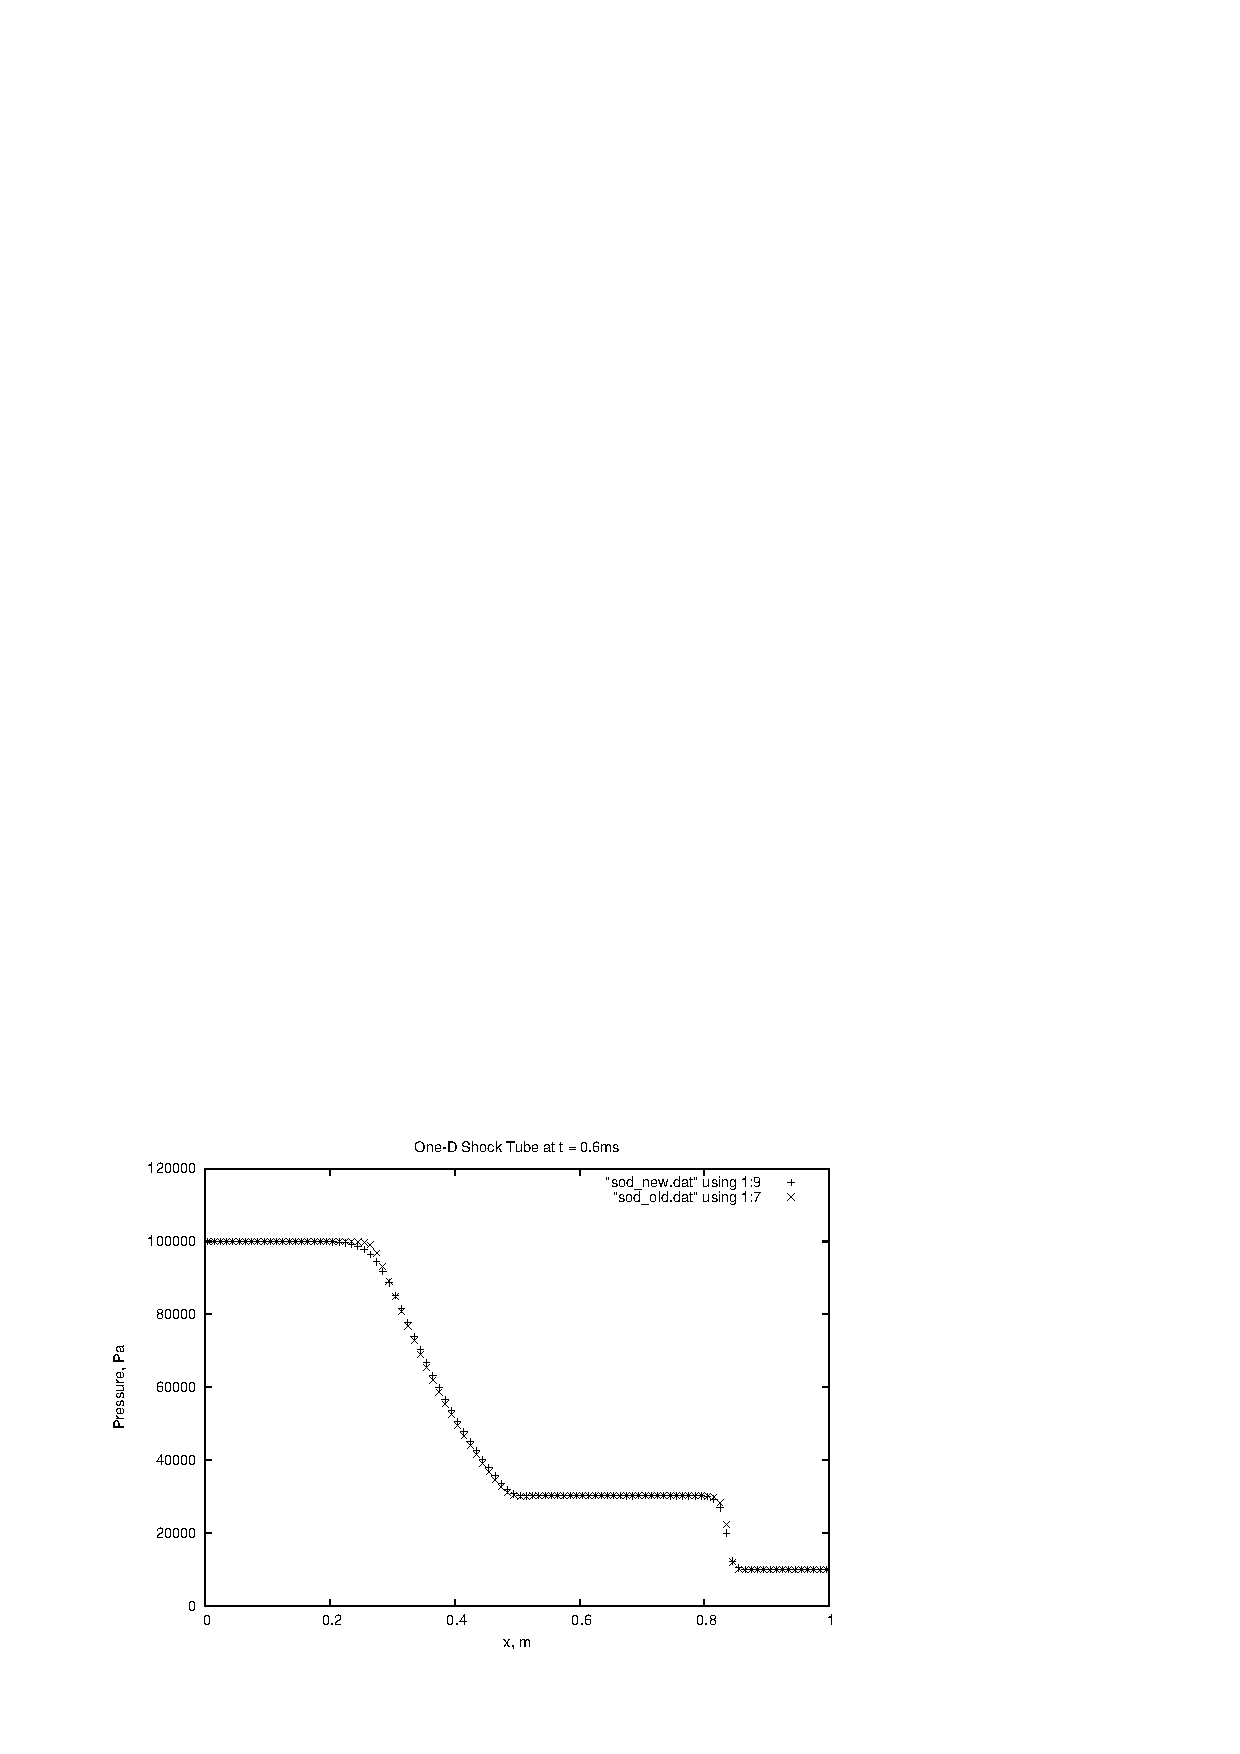
\includegraphics[width=0.5\textwidth,viewport=51 58 400 298,clip=true]{../3D/sod/sod_p.pdf} &
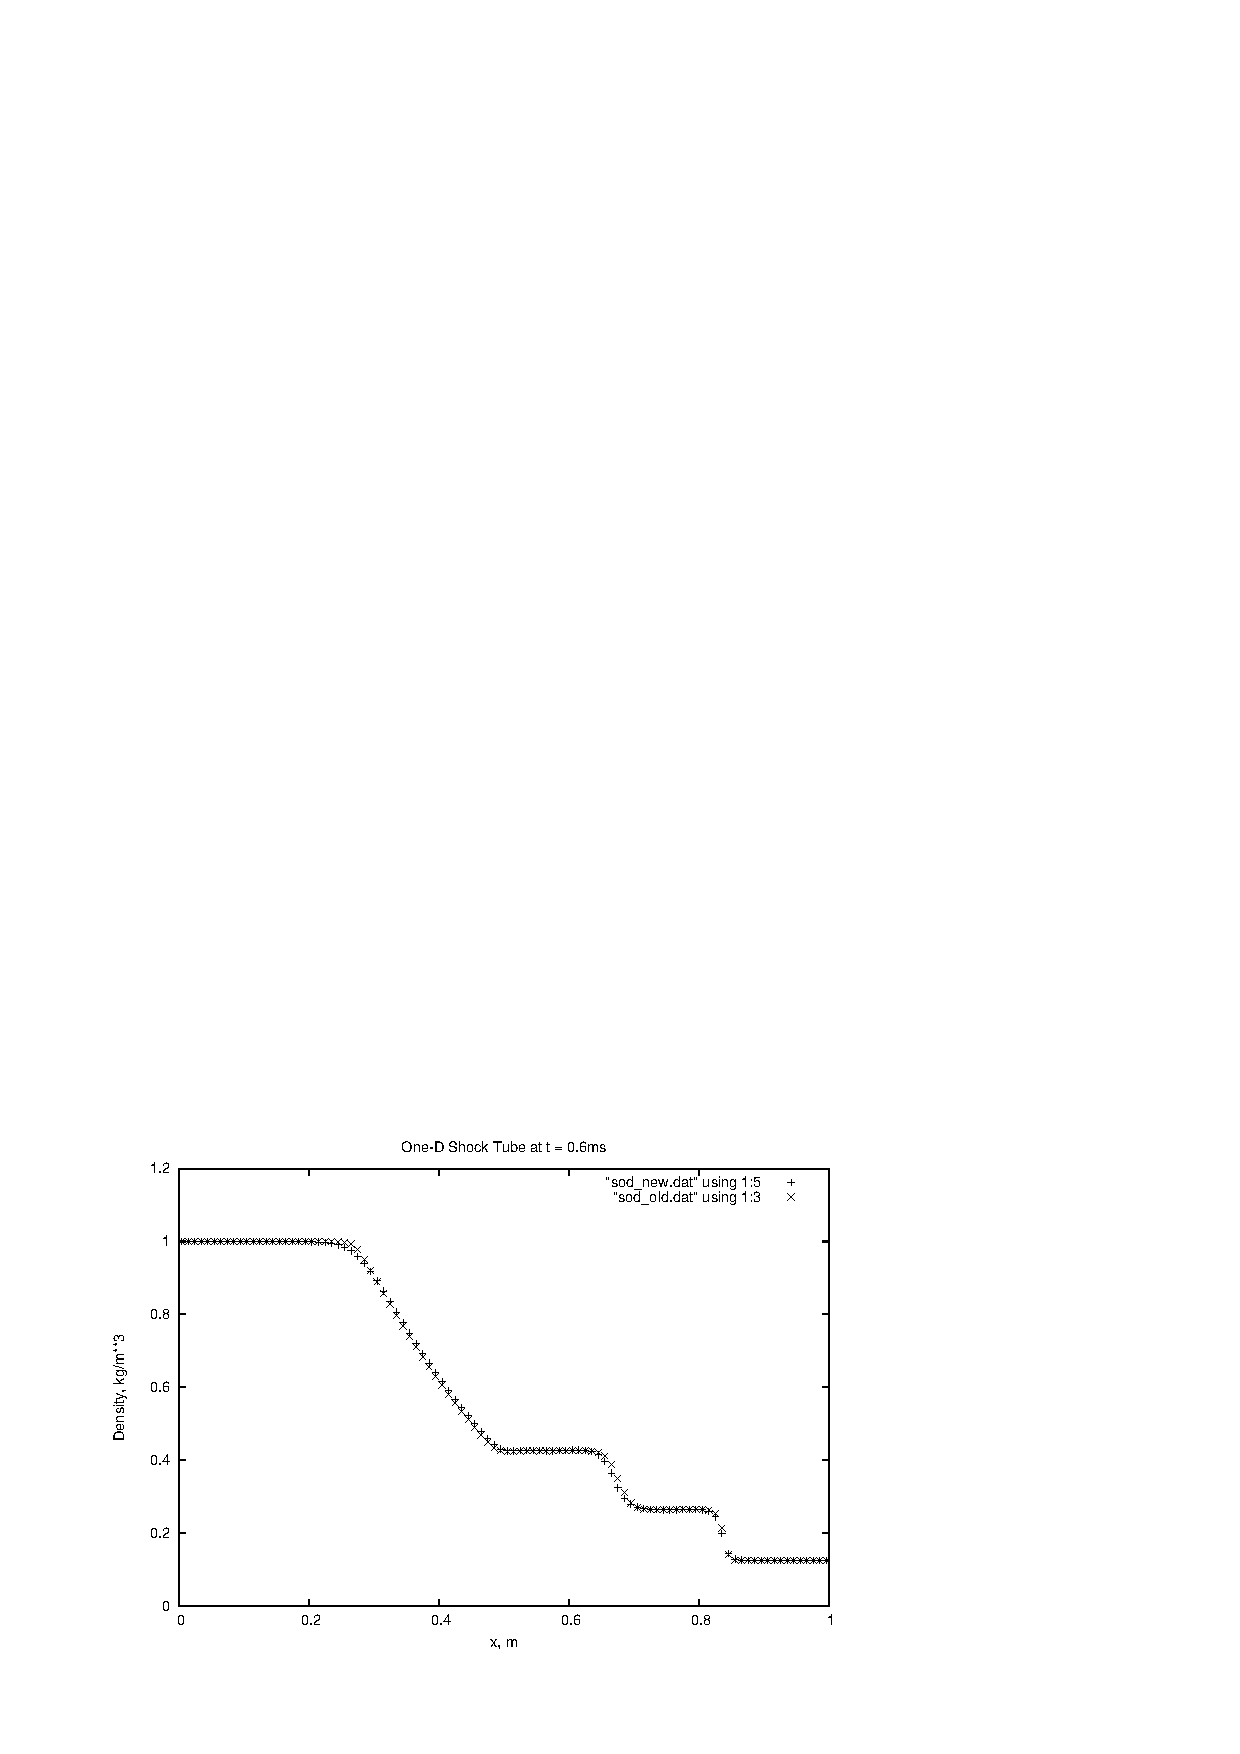
\includegraphics[width=0.5\textwidth,viewport=51 58 400 298,clip=true]{../3D/sod/sod_rho.pdf}\\
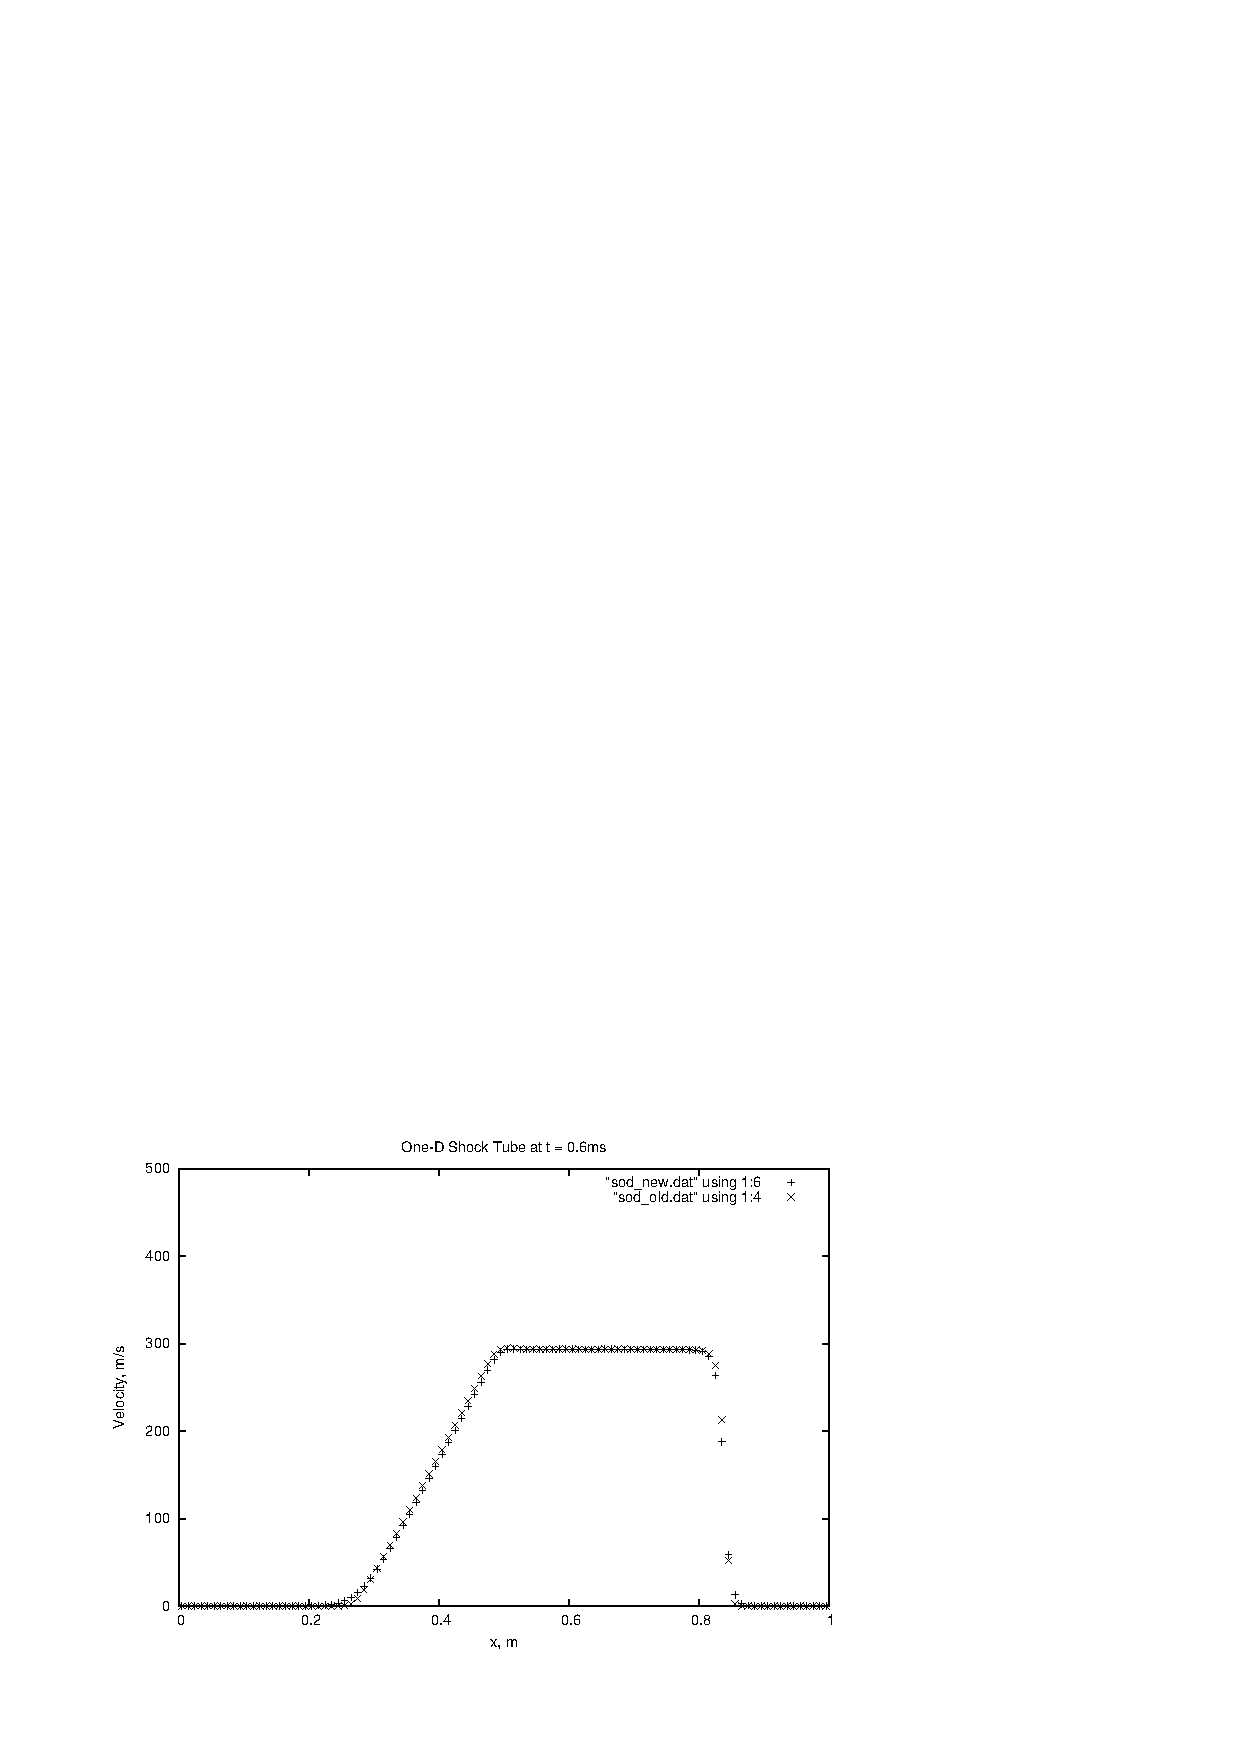
\includegraphics[width=0.5\textwidth,viewport=51 58 400 298,clip=true]{../3D/sod/sod_u.pdf} &
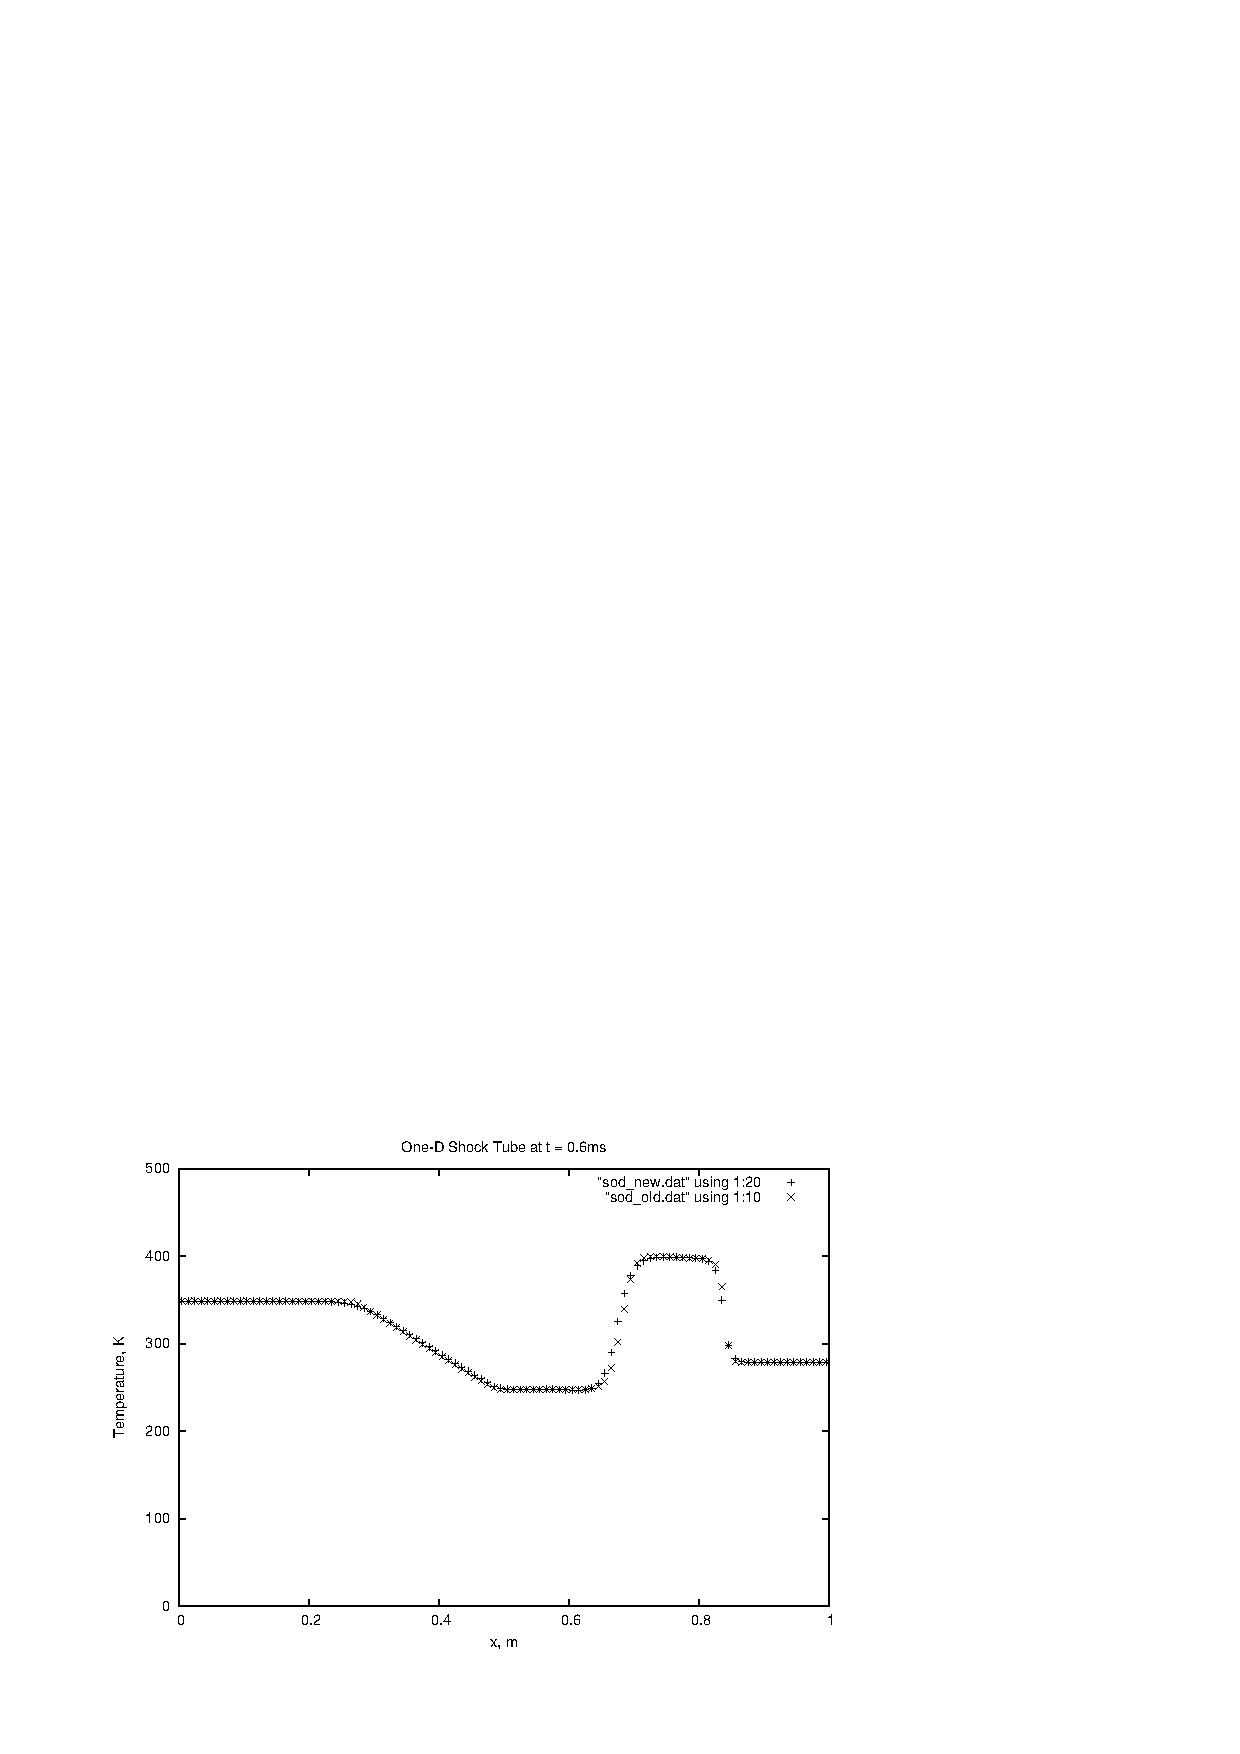
\includegraphics[width=0.5\textwidth,viewport=51 58 400 298,clip=true]{../3D/sod/sod_T.pdf}
\end{tabular}
\caption{Flow properties along the duct for the Sod shock tube problem.}
\label{sod-3d-profiles-fig}
\end{figure}

\newpage
\subsection{Input script (.py)}
\label{sod-3d-py-file}
\topbar
\lstinputlisting[language={}]{../3D/sod/sod.py}
\bottombar

\newpage
\subsection{Shell script}
\label{sod-3d-sh-files}
\topbar
\lstinputlisting[language={}]{../3D/sod/sod_run_and_plot.sh}
\bottombar

\subsection{Notes}
\begin{itemize}
\item None
\end{itemize}
